\documentclass[12pt]{upenndiss}

\usepackage[includeheadfoot,margin=1in]{geometry}

% \usepackage{fancyhdr}
% \pagestyle{fancy}
%\chead{\textbf{Ahern} -- Representative Publication One}


%bibliography
\usepackage{natbib}
\bibpunct[:]{(}{)}{,}{a}{}{,}

% tables and figures
\usepackage{booktabs}
\usepackage{graphicx}
\usepackage{floatrow}
\usepackage{multirow}
\usepackage{enumitem}
\newfloatcommand{capbtabbox}{table}[][\FBwidth]
\setlist{noitemsep}

% Add packages and definitions you want to use here:
\usepackage{times}
\usepackage{multirow,sectsty}
\usepackage{setspace}
\usepackage{subfigure,graphicx}
\usepackage{amsmath,amsthm,amsfonts, amssymb}
\theoremstyle{definition} \newtheorem{definition}{Definition} 
\usepackage{linguex}
\usepackage[english,greek]{betababel}
\usepackage{tikz-qtree}
\usepackage{tikz}
\usetikzlibrary{arrows,automata,chains,matrix,positioning,scopes}

\usepackage[normalem]{ulem}

\usepackage{pdfpages}


\usepackage{epigraph}
\usepackage{hyperref}

 \usepackage[only, llbracket,rrbracket]{stmaryrd}
 \newcommand{\sem}[1]{\ensuremath{\{ #1 \} }}
 \newcommand{\pair}[1]{\ensuremath{\langle #1 \rangle}}
 \newcommand{\la}{\ensuremath{\lambda}}
 \newcommand{\inter}[1]{\ensuremath{\llbracket#1\rrbracket}}

\newcommand*\circled[1]{\tikz[baseline=(char.base)]{
            \node[shape=circle,draw,inner sep=2pt] (char) {#1};}}


\newcommand{\comm}[1]{}
\long\def\symbolfootnote[#1]#2{\begingroup%
\def\thefootnote{\fnsymbol{footnote}}\footnote[#1]{#2}\endgroup}

\begin{document}

\setcounter{chapter}{1}
\chapter{Jespersen's Cycles}
\label{jespersens-cycles}

\setlength{\epigraphwidth}{.9\textwidth}
\epigraph{The history of negative expressions in various languages makes us witness the following curious fluctuation: the original negative adverb is first weakened, then found insufficient and therefore strengthened, generally through some additional word, and this in its turn may be felt as the negative proper and may then in course of time be subject to the same developments as the original word. \citep[4]{jespersen:1917}}

Originally coined by \cite{dahl:1979}, the term \emph{Jespersen's cycle} is often used in reference to the observation cited above. It is certainly the most quoted aspect of Jespersen's \citeyearpar{jespersen:1917} seminal work, which prefigures many of the current empirical and theoretical issues in the study of negation (cf. \citealt{horn:1989}). Yet, this passage is also interpreted in two very distinct ways. This fundamental ambiguity stems from the fact that Jespersen noted both \emph{formal} and \emph{functional} patterns in the expression of sentential negation over time.\footnote{Sentential negation refers to the semantic property of negating an entire proposition, not just some subpart. It can be distinguished from morphological (e.g. \emph{un-}, \emph{non-}) and constituent negation (e.g. \emph{John might have not understood}) using several diagnostics such as tag questions \citep{klima1964}  and performative paraphrases \citep{payne1985}. Sentential negation is also distinct from but related to the syntactic notion of standard negation \citep{miestamo2005}, which refers to constructions that can reverse the truth value of a proposition.} Both patterns can be conceived of as cycles in their own right. That is, we can find a series of transitions from and back to states that are in some sense formally or functionally equivalent. But, the term Jespersen's cycle is often used in one of these two senses or the other, without clear distinction. 

%There are a range of ways to analyze the syntactic structures underlying the formal cycle. As summarized in part by \cite{vanderAuwera2009}, different analyses have suggested varying levels of detail in the number and realization of stages, ranging from three stages  \citep{burridge1983,bernini-ramat1996,haspelmath1997,frisch1997,zanuttini1997,horn:1989,hoeksma1997,horn2001,roberts-roussou2003,vanderAuwera-neuckermans2004,mazzon2004,willis2005,lucas2007,jager2008,wallage2008}, to four stages \citep{dahl:1979,posner1985,schwegler1988,schwegler1990,ladusaw1993,schwenter2005,schwenter2006}, up to five stages \citep{honda2000,beukema1999,vanderAuwera-neuckermans2004,zeijlstra2004}.  


Perhaps even worse, the canonical presentation of what is referred to as Jespersen's cycle conflates these two uses \citep{posner1985,schwegler1988,schwegler1990,ladusaw1993,schwenter2005,schwenter2006}. Where parentheses at the second stage indicate an optional post-verbal element that is characterized as being emphatic, the following stages are posited.

\begin{center}
\begin{enumerate}
     \item \textsc{\textcolor{red}{neg V}}
    \item  \textsc{\textcolor{red}{neg V} \textcolor{blue}{(neg)}}
    \item \textsc{\color{blue} neg V neg}
    \item \textsc{\color{green} V neg}
\end{enumerate}
\end{center}
This chapter is devoted to defining and distinguishing the two uses of the term intertwined in this representation, which we will call the formal and functional Jespersen cycles. In short, the distinction is between changes in the forms of negation available and changes in how those forms are used to signal meaning, respectively.  Our goal is to clarify the relationship between the two cycles and what would count as an explanation of each.

First, we outline the formal aspects of how negation is expressed at the stages of the formal cycle. We provide a historical description of the structural forms that express negation at different points in the history of English, and compare this trajectory with that of French to emphasize particular aspects of the formal cycle. Second, we outline the function of those forms at different stages of the functional cycle. We provide a historical description of the functions of the different forms at points in the history of both English and French, noting the relationship between optionality and these different functions. We also note the logical relationship between the two cycles: the formal cycle entails the functional cycle, but not vice versa. Third, in light of our definitions and the logical relationship between the two cycles, we discuss two ways of conceptualizing the causes of the cycles and the potential role of syntactic acquisition and pragmatic use in both. 

While the main motivation of this chapter is terminological, distinguishing between the two kinds of cycles has an important consequence. Given the logical relationship between the two cycles, an explanation of the formal cycle requires an explanation of the functional cycle. This informs the structure of the dissertation. Since an explanation of the functional cycle must be our first priority, we begin in Part I by pursuing such an explanation. In Chapter 3 we present a mathematical framework for understanding how different functional meanings are signaled in populations over time. In Chapter 4 we apply this framework to model the functional cycle in the history of English.  With this in place, in Part II we turn to the formal cycle. In Chapter 5 we evaluate a model of syntactic acquisition and the role it might play in an explanation of the formal cycle. In Chapter 6 we consider the possibility that stochastic processes may lead to the transitions in the formal cycle. So, our goal in this chapter is to set the foundation for the rest of the dissertation by clarifying the distinction between the two kinds of cycles.


\section{The Formal Cycle}

The formal cycle is defined in terms of the forms that are used to express negation over time, and consists of two transitions. At the start of the formal cycle, a single element is used to express negation. The first transition occurs when this single element is supplemented by additional lexical material. The second transition occurs when the original negative element is subsequently lost, leaving the added lexical material as the only expression of negation. In the most general sense, the formal cycle occurs when the form of negation becomes more and then less complex.  It is cyclic in the sense that the forms of negation at the start and end of the cycle are of equal formal complexity. 

This can be shown schematically as in Figure \ref{formal-cycle}, where the vertical axis represents the degree of formal complexity. The first transition takes place from \circled{1} to \circled{2} with the addition of material. The second transition takes place from \circled{2} back to \circled{1} with the loss of material. The addition of material leads to an increase in formal complexity of negation and the loss of material leads to a decrease. The formal cycle is then just a cycle from and back to a less complex form of negation: negation is expressed by some stuff, then more stuff, then less stuff.

%\footnote{We could perhaps be a bit more general by replacing one and two in Figure \ref{formal-cycle} with \circled{$n$} and \circled{$n+1$}, respectively, where $n$ indicates the number of elements used to express negation.} 

\begin{figure}
% Modified from:
% A simple cycle
% Author : Jerome Tremblay
\begin{tikzpicture}
	% Define margin to offset
	\def \margin {8}
	% Draw nodes
	\node[draw,circle] at ({90}:3) {2};
	\node[draw,circle] at ({270}:3) {1};
	% Draw arcs
	\draw[->, >=latex] ({270 - \margin}:3) arc ({270 - \margin}:{90 + \margin}:3);
	\draw[->, >=latex] ({90 - \margin}:3) arc ({90 - \margin}:{-90 + \margin}:3);
	% Draw complexity axis
	\draw[->, >=latex] (-5,-3) -- (-5,3);
	\node[align=center,text width=2cm] at (-6.25, 0) {Formal complexity};
\end{tikzpicture}
\caption{The formal Jespersen cycle}
\label{formal-cycle}
\end{figure}

For example, Jespersen noted that in the history of several European languages, including English and French, a pre-verbal negative element is supplemented by a post-verbal element, and the pre-verbal element is subsequently lost.  This can be shown schematically as in Figure \ref{formal-cycle-spiral} where the different forms of negation are arranged according to formal complexity on the vertical axis and time along the horizontal axis. At both the start and the end of the formal cycle a single element expresses negation. Intuitively, if we abstract away from the structural realization of the forms as pre- or post-verbal, then Figure \ref{formal-cycle-spiral} maps onto Figure \ref{formal-cycle}. The curious fluctuation in form that Jespersen noted simply becomes a closed orbit through the space of formal complexity.

\begin{figure}
\begin{center}
\begin{tikzpicture}[->,>=stealth',shorten >=1pt,auto,node distance=3cm]
  \node (A)      {\textsc{\textcolor{red}{neg V}}};
  \node (B) [above right of=A]  {\textsc{\color{blue} neg V neg}};
  \node (C) [below right of=B] {\textsc{\color{green} V neg}};
  \node (D) [left of=A] {};
  \node (E) [above of=D] {};
\path[->] (A)  edge node {} (B)
  (B) edge node {} (C);
	% Draw axes
    \draw[->] (-1.5,0) -- (-1.5,2);
  \node[align=center, text width=2cm] at (-2.75, 1) {Formal complexity};
    \draw[->] (0,-1) -- (4,-1);
    \node at (2,-1.5) {Time};
\end{tikzpicture}
\end{center}
\caption{The realization of the formal cycle in English and French}
\label{formal-cycle-spiral}
\end{figure}

We see the first stage of the formal cycle in the history of English with the pre-verbal \emph{\textcolor{red}{ne}} in Old English, which expresses sentential negation alone.

\exg. Ic \textcolor{red}{ne} secge\\
      I \textsc{neg} say\\
      (Old English)


This is followed by a stage of embracing or bipartite negation where a post-verbal negative element is added. This is seen in Middle English, where \emph{\textcolor{blue}{ne}} is supplemented by \emph{\textcolor{blue}{not}}.


\exg. I \textcolor{blue}{ne} seye \textcolor{blue}{not}\\
      I \textsc{neg} say \textsc{neg}\\
      (Middle English)

There are several sources that these additional elements are drawn from, most notably from \emph{negative polarity items}, overwhelmingly the set of \emph{minimizers} (e.g. ``not a drop'', ``not a hair'') and \emph{generalizers} (e.g. ``not ever'', ``not at all'', \citealt{horn:1989}). For example, in the case of English, \emph{not} comes from Old English \emph{nawiht} (\emph{literally} ``no thing, creature, being''). Other sources include, indefinite pronouns (e.g. ``no one''), negative adverbs (e.g. ``never'', cf. \citealt{horn:1989,vanGelderen2008negative}), negative verbs (e.g. ``refuse", ``deny", ``reject", ``avoid", ``fail", and ``lack",  \citealt{givon1978}), and the concatenation of negative and existential verbs \citep{croft1991}.


In light of this broad range of sources, it is important to note that the first transition need not consist of the addition of a post-verbal element. For example, in modern African American Vernacular English, negation can be supplemented by a pre-verbal element \emph{eem}, which can express negation in its own right \citep{jones2015}.

\ex. You do\textcolor{blue}{n't eem} know.

\ex. You \textcolor{blue}{eem} know.

As \cite{jones2015} notes, this form comes from but is arguably distinct from \emph{even}.

\ex.  \# \textcolor{blue}{eem} numbers

Importantly, it is the formal status rather than the structural position that is relevant. Given the range of sources for additional negative elements, this is not surprising.  But, it bears emphasis that the transition from pre- to post-verbal negation is not the only path through the formal cycle.  The transition could just as well have been from post- to pre-verbal negation or from and back to pre-verbal negation. It is a contingent historical fact, arising from the syntax of  English and the source of the additional  material, rather than some necessary property of the formal cycle. 

The final stage in the formal cycle is a return to a single negative element. This is seen in Early Modern English, where the preverbal element in \emph{\textcolor{blue}{ne...not}}  is lost, leaving the post-verbal \emph{\textcolor{green}{not}}  as the sole negative element.

\exg. I say \textcolor{green}{not}\\
      I say \textsc{neg}\\
      (Early Modern English)

The emergence of  \emph{do}-support in Early Modern English yields a state parallel to Old English with a sole pre-verbal negator:

\exg. I do \textcolor{red}{not} say\\
      I do \textsc{neg} say\\
      (Present-day English)

The contraction of negation offers an even closer parallel to Old English where \emph{ne} contracted with several verbs (e.g. \emph{ne be} $\rightarrow$ \emph{nis}).

\exg. I do\textcolor{red}{n't} say\\
      I do-\textsc{neg} say\\
      (Present-day English)

But, however suggestive these further developments are, they are not necessary components of the formal cycle.  \citet[10]{jespersen:1917} himself noted the uniqueness of these developments, which he attributed to a tendency to place negation at the beginning of the sentence to avoid confusion. As he put it, the effect of post-verbal negation in German results in a kind of semantic garden path.\footnote{Translation, check with Florian: Living is not the highest good (lit. The living is the good highest not)}

\begin{quote}
[T]he hearer or reader is sometimes bewildered at first and thinks that the sentence is to be understood in a positive sense, till suddenly he comes upon the \emph{nicht}, which changes everything; see, for instance ``Das leben ist der g\"{u}ter h\"{o}chstes nicht."
\end{quote}
Yet, despite this purported tendency, the majority of languages that Jespersen noted, including his native Danish, persist in a perplexing state of post-verbal negation. This can only be taken as further evidence that we ought to interpret the implications of Jespersen's observation in formal rather than structural terms. It matters how much stuff is used to express negation, not where that stuff is.

% The transition from purely post-verbal to purely pre-verbal negation is certainly not necessary. For example, German went through a formal cycle in (cf. CHECK \cite{jager2008}), but negation remains purely post-verbal.

% \footnote{The increasing preference of n't over not in colloquial use is illustrated by the use of not contractions of American presidents from Kennedy to Bush. While Kennedy and Nixon still used the uncontracted form not in the majority of cases (during public debates), Bush Sr. and Clinton used this form in only in 14-17\% of all cases (Yaeger-Dror \& Hall-Lew (2002)}

Given the stages of the formal cycle in the history of English, it is useful to give them some historical context. The stages are summarized in Figure \ref{english-timeline}. The horizontal axis represents years in the common era. Immediately above the horizontal axis are commonly-used terms for historical periods: Old English (\emph{ca.} 400-1175 CE), Middle English (\emph{ca.}1175-1450 CE), Early Modern English (\emph{ca.} 1450-1650 CE), and Modern English (\emph{ca.} 1650-Present CE). Above these general time periods are the spans of the different forms of negation.  From Old to Early Modern English we make a full formal cycle from and back to a single negative element. We also see the transition at the end of the formal cycle from post- back to pre-verbal negation in Modern English. 

Below the axis are rough historical anchors that offer a general sense of the historical periods: Beouwulf, the Old English epic poem written some time between 700-1050 CE; Chaucer, the Late Middle English author who is widely-credited as the first to write in the vernacular language of his day, from around 1350-1400 CE; and Shakespeare, the noted dramatist and playwright, from around 1550-1650 CE.


\begin{figure}
\resizebox{\linewidth}{!}{% 
     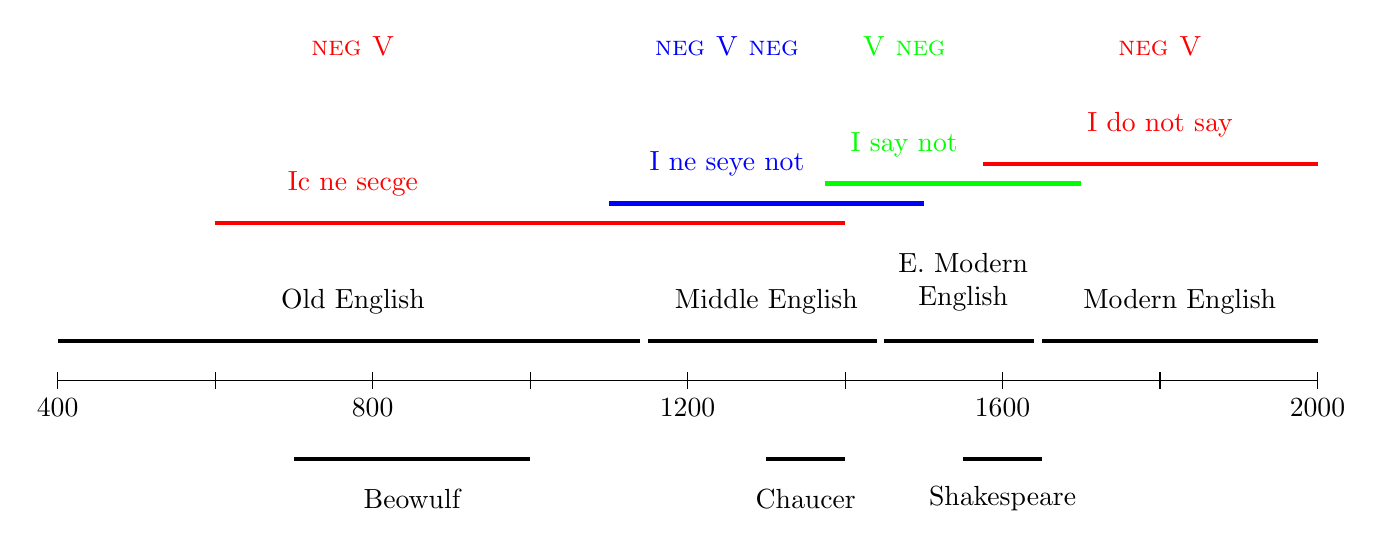
\begin{tikzpicture}
%draw horizontal line
\draw (0,0) -- (16,0);
%draw ticks
\foreach \x in {0, 2, 4, 6, 8, 10, 12, 14, 16}{
   \draw (\x,3pt) -- (\x,-3pt);
}
%draw tick dates
\draw (0,0) node[below=3pt] { 400 } node[above=10pt] { };
\draw (4,0) node[below=3pt] { 800 } node[above=10pt] { };
\draw (8,0) node[below=3pt] { 1200 } node[above=3pt] { };
\draw (12,0) node[below=3pt] { 1600 } node[above=3pt] { };
\draw (16,0) node[below=3pt] { 2000 } node[above=3pt] {  };
% Historical examples
\draw [ultra thick] (3,-1) to (6,-1);
\draw (4.5, -1.5) node {Beowulf};
\draw [ultra thick] (9,-1) to (10,-1);
\draw (9.5, -1.5) node {Chaucer};
\draw [ultra thick] (11.5,-1) to (12.5,-1);
\draw (12, -1.5) node {Shakespeare};
% Add historical languages
% Old English : 400-1175
% Middle English : 1175-1450
% E. Modern English : 1450-1650
% Modern English : 1650-Present
\draw [ultra thick] (0,.5) to (7.4,.5);
\draw (3.75, 1) node {Old English};
\draw [ultra thick] (7.5,.5) to (10.4,.5);
\draw (9, 1) node {Middle English};
\draw [ultra thick] (10.5,.5) to (12.4,.5);
\draw (11.5, 1.25) node[text width=2cm,align=center] {E. Modern English};
\draw [ultra thick] (12.5,.5) to (16,.5);
\draw (14.25, 1) node {Modern English};
% draw ticks for historical examples
% ne 		: 400-1300
% ne..not	: 1100-1400
% not		: 1350-1700
% do not 	: 1500-2000
\draw [ultra thick,red] (2,2) to (10,2);
\draw (3.75, 2.5) node[red] {Ic ne secge};
\draw [ultra thick,blue] (7,2.25) to (11,2.25);
\draw (8.5, 2.75) node[blue] {I ne seye not};
\draw [ultra thick,green] (9.75,2.5) to (13,2.5);
\draw (10.75, 3) node[green] {I say not};
\draw [ultra thick, red] (11.75,2.75) to (16,2.75);
\draw (14, 3.25) node[red] {I do not say};
% draw negative forms
\draw (3.75,4) node [above] {\textsc{\color{red} neg V}};
\draw (8.5,4) node [above] {\textsc{\color{blue} neg V neg}};
\draw (10.75,4) node [above] {\textsc{\color{green} V neg}};
\draw (14,4) node [above] {\textsc{\color{red} neg V}};
\end{tikzpicture}
}
\caption{Timeline of negation in the history of English}
\label{english-timeline}
\end{figure}

The history of negation in French offers a parallel to the formal cycle in English, although the exact details of the timeline are not without dispute (cf. \citealt{martineau-mougeon2003}).  The Old French pre-verbal \emph{\textcolor{red}{ne}} becomes Middle French \emph{\textcolor{blue}{ne...pas}}, and subsequently Modern Colloquial French post-verbal \emph{\textcolor{green}{pas}}.

\exg. Jeo \textcolor{red}{ne} dis\\
      I \textsc{neg} say\\
      (Old French)

\exg. Je \textcolor{blue}{ne} dis \textcolor{blue}{pas}\\
      I \textsc{neg} say \textsc{neg}\\
      (Middle French)

\exg. Je dis \textcolor{green}{pas}\\
      I say \textsc{neg}\\
      (Modern Colloquial French)

Again, it is useful to provide some historical context. The stages of the formal cycle in the history of French are summarized in Figure \ref{french-timeline}. Immediately above the horizontal axis are commonly-used terms for historical periods: Old French (\emph{ca.} 900-1350 CE), Middle French (\emph{ca.}1350-1600 CE), Classical French (\emph{ca.} 1600-1700 CE) , and Modern French (\emph{ca.} 1700-Present CE). Above these general time periods are the spans of the different forms of negation.  From Old to Modern French we make a full formal cycle from and back to a single negative element.

Below the axis are rough historical anchors that offer a general sense of the historical periods: Charlemagne, the first Holy Roman Emperor from 750-800 CE; the Hundred Years' War from roughly 1350-1450 CE; Voltaire, the Enlightenment author and satirist from roughly 1700-1800 CE.


\begin{figure}
\resizebox{\linewidth}{!}{% 
     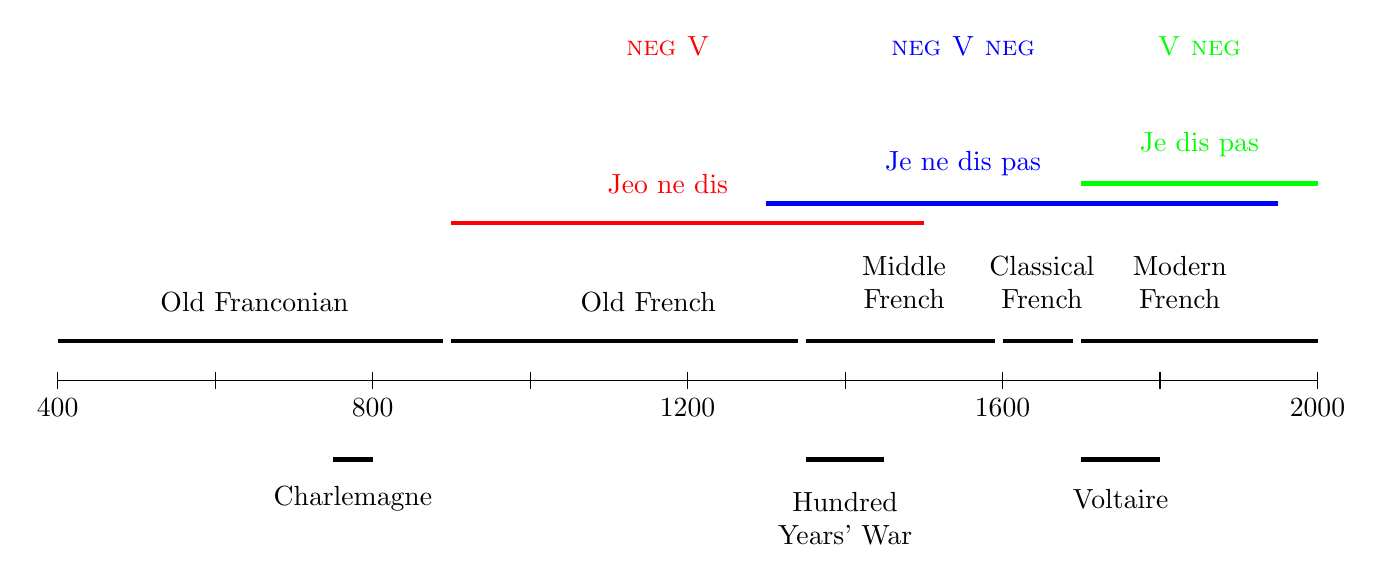
\begin{tikzpicture}
%draw horizontal line
\draw (0,0) -- (16,0);
%draw ticks
\foreach \x in {0, 2, 4, 6, 8, 10, 12, 14, 16}{
   \draw (\x,3pt) -- (\x,-3pt);
}
%draw tick dates
\draw (0,0) node[below=3pt] { 400 } node[above=10pt] { };
\draw (4,0) node[below=3pt] { 800 } node[above=10pt] { };
\draw (8,0) node[below=3pt] { 1200 } node[above=3pt] { };
\draw (12,0) node[below=3pt] { 1600 } node[above=3pt] { };
\draw (16,0) node[below=3pt] { 2000 } node[above=3pt] {  };
% Add historical languages
% Old Franconian : 400-900
% Old French : 900-1350
% Middle French : 1350-1600
% Classical French : 1600-1700
% Modern French : 1700-Present
\draw [ultra thick] (0,.5) to (4.9,.5);
\draw (2.5, 1) node {Old Franconian};
\draw [ultra thick] (5,.5) to (9.4,.5);
\draw (7.5, 1) node {Old French};
\draw [ultra thick] (9.5,.5) to (11.9,.5);
\draw (10.75, 1.25) node[text width=2cm,align=center] {Middle French};
\draw [ultra thick] (12,.5) to (12.9,.5);
\draw (12.5, 1.25) node[text width=2cm,align=center] {Classical French};
\draw [ultra thick] (13,.5) to (16,.5);
\draw (14.25, 1.25) node[text width=2cm,align=center] {Modern French};
% draw ticks for historical examples
% ne 		: 400-1300
% ne..not	: 1100-1400
% not		: 1350-1700
% do not 	: 1500-2000
\draw [ultra thick,red] (5,2) to (11,2);
\draw (7.75, 2.5) node[red] {Jeo ne dis};
\draw (7.75,4) node [above] {\textsc{\color{red} neg V}};
\draw [ultra thick,blue] (9,2.25) to (15.5,2.25);
\draw (11.5, 2.75) node[blue] {Je ne dis pas};
\draw (11.5,4) node [above] {\textsc{\color{blue} neg V neg}};
\draw [ultra thick,green] (13,2.5) to (16,2.5);
\draw (14.5, 3) node[green] {Je dis pas};
\draw (14.5,4) node [above] {\textsc{\color{green} V neg}};
%\draw (14,4) node [above] {\textsc{\color{red} neg V}};
% Historical examples
\draw [ultra thick] (3.5,-1) to (4,-1);
\draw (3.75, -1.5) node {Charlemagne};
\draw [ultra thick] (9.5,-1) to (10.5,-1);
\draw (10, -1.75) node[text width=2.2cm,align=center] {Hundred Years' War};
%\draw [ultra thick] (11,-1) to (12,-1);
%\draw (11.5, -1.5) node {Rabelais};
\draw [ultra thick] (13,-1) to (14,-1);
\draw (13.5, -1.5) node {Voltaire};
\end{tikzpicture}
}
\caption{Timeline of negation in the history of French}
\label{french-timeline}
\end{figure}

\cite{hansen-visconti2009,hansen-visconti2012} note that negation in Louisiana Creole French negation is purely pre-verbal. Of course, this observation comes with the caveat that no conclusions about the future of French can be drawn from this change.

%Although, \cite{hansen-visconti2009,hansen-visconti2012} also note that the post-verbal negator \emph{pas} appears pre-verbally in embedded infinitives \citep{martineau1994}

\exg. Mo \textcolor{red}{pa} di \\
      I \textsc{neg}  say\\
      (Louisiana Creole French)

But again, even if such developments were readily apparent, they would not constitute a necessary component of the formal cycle.
      
Thus, the crucial components of the formal cycle are a transition from one negative element to two, and eventually back to one. For the specific case of English, as well as French, the formal cycle is realized as a transition from pre-verbal to embracing to post-verbal negation. We can represent these transitions schematically as follows.

\begin{center}
\begin{enumerate}
     \item \textsc{\textcolor{red}{neg V}}
    \item \textsc{\color{blue} neg V neg}
    \item \textsc{\color{green} V neg}
\end{enumerate}
\end{center}

Note that these stages are not mutually exclusive. That is, there are transitions between these stages \citep{vanderAuwera2009}.  This captures the theoretical intuition that diachronic change is rarely a dramatic shift. Where parentheses are taken to indicate optionality, the stages can be represented as the following.

\begin{center}
\begin{enumerate}
     \item \textsc{\textcolor{red}{neg V}}
    \item  \textsc{\textcolor{red}{neg V} \textcolor{blue}{(neg)}}
    \item \textsc{\color{blue} neg V neg}
    \item \textsc{\textcolor{blue}{(neg)}  \textcolor{green}{V neg}}    
    \item \textsc{\color{green} V neg}
\end{enumerate}
\end{center}
This more articulated model also comes closer to the diachronic facts. For example, in Late Middle English, all the forms of negation are used contemporaneously: purely pre-verbal, embracing, and post-verbal negation co-occur for a brief period in time. For the moment then, we can take this as the abstract trajectory of the formal cycle over time. 

Importantly, an explanation of the formal cycle in English must consist of two components: it must provide the conditions for the transition from pre-verbal to embracing negation as well as the conditions for the transition from embracing to post-verbal negation. It should be noted that criterion for such explanations can be both qualitative and quantitative. That is, an explanation of the formal cycle can predict both \emph{that} a transition will occur as well as \emph{how} it will occur. In what follows, we will use both kinds of criteria in evaluating models as explanations of change. With this definition of the formal cycle in place, along with what would constitute an explanation for its instantiation in the history of English, we turn to the functional cycle.

%This also occurs synchronically in modern Brazilian Portuguese \citep{schwenter2005, schwenter2006}. 

\section{The Functional Cycle}

%If the formal cycle is defined by the forms of negation, then the functional cycle is defined by the functions that those forms are put to. It is about how and how many forms are used to mean different things. At the first stage of the cycle one form is generally used to express negation, often characterized as plain negation. Another set of forms is used to express negation in a semantically stronger sense, often characterized as being more emphatic. The first transition in the functional cycle occurs when one of the semantically stronger forms weakens to a strength intermediate between plain and emphatic negation. Thus, at the second stage of the functional cycle the available forms of negation are used to make three functional distinctions. The second transition occurs when the intermediate form weakens even further, coming to have the strength of plain negation, and the original form of plain negation is lost. In the most general sense, the functional cycle occurs when one form of plain negation is replaced by another. It is cyclic in the sense that the number of functionally distinct forms of negation increases then decreases. 

If the formal cycle is defined by the forms of negation, then the functional cycle is defined by the function that those forms are put to. It is about how and how many forms are used to mean different things. At the first stage of the functional cycle a single form is generally used to express negation, often characterized as plain negation. The functional cycle begins with the introduction of another form that is used to express negation in a semantically stronger way, often characterized as being more emphatic. The functional cycle progresses as this new stronger form increases in frequency, weakens, and replaces the original negative form. In the most general sense, the functional cycle occurs when the form of plain negation is replaced by another form. It is cyclic in the sense that the number of functionally distinct forms of negation increases then decreases.

This can be shown schematically as in Figure \ref{functional-cycle} where the vertical axis represents the number of functionally distinct forms of negation. The addition of a new form increases the number of distinctions from \circled{1} to \circled{2}, and the loss of the original form decreases the number of distinctions from \circled{2} back to \circled{1}. However, we should note that Figure \ref{functional-cycle} does not convey all of the necessary information about the functional cycle.

% \footnote{ADD: there aren't JUST two functional distinctions. There are always means of augmenting plain negation to make it emphatic. It might be better to say 2-3-2.}

\begin{figure}
\begin{tikzpicture}
	% Define margin to offset
	\def \margin {8}
	% Draw nodes
	\node[draw,circle] at ({90}:3) {2};
	\node[draw,circle] at ({270}:3) {1};
	% Draw arcs
	\draw[->, >=latex] ({270 - \margin}:3) arc ({270 - \margin}:{90 + \margin}:3);
	\draw[->, >=latex] ({90 - \margin}:3) arc ({90 - \margin}:{-90 + \margin}:3);
	% Draw complexity axis
	\draw[->, >=latex] (-5,-3) -- (-5,3);
	\node[align=center,text width=3cm] at (-6.75, 0) {Functional distinctions};
\end{tikzpicture}
\caption{The functional Jespersen cycle}
\label{functional-cycle}
\end{figure}

Namely, the functional cycle does not hold for just any pair of semantic distinctions. Rather, the incoming form is semantically stronger than the incumbent form. We can more accurately represent the details of the functional cycle as  in Figure \ref{functional-cycle-detail}, where the vertical axis represents semantic strength and the horizontal axis represents time. The original form is supplemented with an additional form that is semantically stronger and this new form weakens over time as it replaces the original from. 

%\footnote{Note that this does not preclude other forms of negation. There are always means for augmenting plain negation to make it emphatic (e.g. `at all', `ever', see \citet[258]{israel2011} and \citet{horn:1989} for incomplete but substantial lists). Crucially the form that is introduced is \emph{more} emphatic than plain negation, but not the only such form.} 

\begin{figure}
\begin{center}
\begin{tikzpicture}[->,>=stealth',shorten >=1pt,auto,node distance=3cm]
  \node[draw,circle] (A)      {1};
  \node[draw,circle] (B) [above right of=A]  {2};
  \node[draw,circle] (C) [below right of=B] {2};
  \node[draw,circle] (D) [below right of=A] {1};
\path[->] (A)  edge node {} (D)
  (B) edge node {} (C);
	% Draw axes
    \draw[->] (-1.5,-2.5) -- (-1.5,2.5);
  \node[align=center, text width=2cm] at (-2.75, 0) {Semantic strength};
    \draw[->] (0,-3) -- (4,-3);
    \node at (2,-3.5) {Time};
%  \node[align=1enter, text width=2cm] at (-2.75, 1) {Formal complexity};
\end{tikzpicture}
\end{center}
\caption{The functional Jespersen cycle in more detail}
\label{functional-cycle-detail}
\end{figure}

The stronger negative form is often a result of elements being added to the original plain form.  For example, in the history of English and French a pre-verbal element is supplemented by a post-verbal element, which strengthens negation. The meaning of the combined pre- and post-verbal elements weakens over time, and the two elements come to have the same force as the original pre-verbal element in isolation. This can be shown schematically as in Figure \ref{functional-cycle-spiral} where the different forms are arranged according to semantic strength along the vertical axis and time along the horizontal axis. If we abstract away from the realization of the particular forms then Figure \ref{functional-cycle-spiral} maps onto Figure \ref{functional-cycle-detail}, which in turn maps onto Figure \ref{functional-cycle}. The curious fluctuation in function that Jespersen noted becomes a particular kind of closed orbit through the space of functional distinctions, which stems from the weakening of negative forms along a semantic dimension.

\begin{figure}
\begin{center}
\begin{tikzpicture}[->,>=stealth',shorten >=1pt,auto,node distance=3cm]
  \node (A)      {\textsc{\textcolor{red}{neg V}}};
  \node (B) [above right of=A]  {\textsc{\color{blue} neg V neg}};
  \node (C) [below right of=B] {\textsc{\color{blue} neg V neg}};
  \node (D) [below right of=A] {\textsc{\textcolor{red}{neg V}}};
\path[->] (A)  edge node {} (D)
  (B) edge node {} (C);
	% Draw axes
    \draw[->] (-1.5,-2.5) -- (-1.5,2.5);
  \node[align=center, text width=2cm] at (-2.75, 0) {Semantic strength};
    \draw[->] (0,-3) -- (4,-3);
    \node at (2,-3.5) {Time};
%  \node[align=1enter, text width=2cm] at (-2.75, 1) {Formal complexity};
\end{tikzpicture}
\end{center}
\caption{The realization of the functional cycle in English and French}
\label{functional-cycle-spiral}
\end{figure}

We see the first stage of the functional cycle in the history of English and French, with pre-verbal \emph{\textcolor{red}{ne}} expressing plain negation.

\exg. Ic \textcolor{red}{ne} secge\\
      I \textsc{neg} say\\
      
\exg. Jeo \textcolor{red}{ne} dis\\
      I \textsc{neg} say\\

The optional addition of a post-verbal element in the embracing forms \emph{\textcolor{blue}{ne...not}} and \emph{\textcolor{blue}{ne...pas}} is used to express a stronger negation.

\exg. I \textcolor{blue}{ne} seye \textcolor{blue}{not}\\
      I \textsc{neg} say \textsc{neg}\\

\exg. Je \textcolor{blue}{ne} dis \textcolor{blue}{pas}\\
      I \textsc{neg} say \textsc{neg}\\

The initial effect of the embracing form, in Jespersen's words \citeyearpar[15]{jespersen:1917}:
%In this case, \emph{not} comes from Old English \emph{nawiht} (\emph{lit.} ``no thing, creature, being''), and indeed has the expected effect. The second stage in the functional cycle in English is evidenced by the use of both \emph{\textcolor{red}{ne}} and \emph{\textcolor{blue}{ne...not}}, where the second has a stronger, emphatic or exaggerative meaning. 

\begin{quotation}
...[I]n most cases the addition serves to make the negative more impressive as being more vivid or picturesque, generally through an exaggeration, as when substantives meaning something very small are used as subjuncts.
\end{quotation}
Despite the evocative phrasing, Jespersen was certainly not the first to notice the trajectory of the functional cycle. It was noted in great detail by both \citet[393]{meillet1912}\footnote{Translation, check with Robin: L� o� l�on avait besoin d�insister sur la n�gation [...] on a �t� conduit � renforcer la n�gation ne ... par quelque autre mot. [...] On sait comment pas a perdu, dans les phrases o� il �tait un accessoire de la n�gation, tout sons sens propre�sens conserv� parfaitement dans le mot isol� pas�, comme d�s lors, pas est devenu � lui seul un mot n�gatif, servant � exprimer la n�gation}
 and \citet[134]{gardiner1904} in French and several other languages.
%\begin{quotation}
%Where we mean to insist upon negation...we are prompted to reinforce the negative \emph{ne}...with some other word....\emph{pas} itself becomes a negative word, used to express negation.
%\end{quotation}

\begin{quotation}
[French \emph{pas} and \emph{point}], from the Latin \emph{passum} and \emph{punctum}, were originally adverbial
accusatives placed at the end of negative sentences for the purpose of emphasis; just
like the English ``not a jot'', ``not a straw''....\emph{Pas} and \emph{point}, and like them the
Demotic B , Coptic AN, next lose their emphasizing force, and become mere adjuncts of
the negative words (French \emph{ne}, Coptic 'N). Last of all, they come themselves to be looked upon as negative words.
\end{quotation}
Indeed, \cite{vanderAuwera2009} suggests that \emph{Meillet's spiral} \citeyearpar[394]{meillet1912} may be the more appropriate term for the functional cycle.\footnote{Translation McMahon 1994, 165 : Les langues suivent ainsi une sorte de d�veloppement en spirale : elles ajoutent des mots accessoires pour obtenir une expression intense : ces mots s�affaiblissent, se d�gradent et tombent au niveau de simples outils grammaticaux ; on ajoute de nouveaux mots ou des mots diff�rents en vue de l�expression ; l�affaiblissement recommence et ainsi sans fin.} 
\begin{quotation}
Thus, languages follow a sort of spiral development: they add extra words to intensify expression; these words fade; decay and fall to the level of simple grammatical tools; one adds new or different words on account of expressiveness; the fading begins again, and so on endlessly.
\end{quotation}

If the functional cycle in English and French begins with the introduction of the optional post-verbal element to create an embracing form that intensifies expression, then it ends when the post-verbal element ceases to be optional. That is, when the post-vebal element becomes obligatory only the embracing form is used, and its intensity fades. This is because the embracing form ceases to be able to signal anything about the distinction between plain and emphatic negation. As \cite{kiparsky-condoravdi:2006} rightly put it, to emphasize everything is to emphasize nothing.  This inverse relation between frequency and informativeness has been argued to underly multiple linguistic phenomena. As forms increase in frequency, they undergo a kind of  \emph{rhetorical devaluation} \citep{dahl:2001}. Simply put, for any form, if it is the only one in use, then it cannot carry any special meaning. There is nothing else to be special in comparison to.

Now that we have defined the formal and functional cycles, there are several important points to be made regarding the relationship between them. First, the effect of one cycle often has implications for the other. For example, the addition of formal material almost always comes with a more restricted and hence stronger meaning.\footnote{The rare exception being truly empty obligatory pleonastic or expletive elements: ``It's raining." Even periphrastic \emph{do}, which is redundant outside of emphatic affirmatives: ``I \textsc{do} want pizza", originally carried some information on its way to becoming obligatory \citep{ecay2015}} This is a natural consequence of how semantic composition proceeds in a generally intersective fashion, to put it set-theoretically. For example, ``a black bear" is certainly more specific, and hence semantically stronger than ``a bear". In the same way, we would expect \emph{\textcolor{blue}{ne...not}} to be more specific in comparison to \emph{\textcolor{red}{ne}}.  This means that the first transition in the formal cycle is virtually guaranteed to coincide with the entirety of a functional cycle, which is indeed what we see in both English and French.

%That is, the functional cycle can occur in the space of a single transition in the formal cycle. This is the case for English and French: the functional cycle ends as the embracing form replaces the pre-verbal element, whereas the formal cycle ends with the subsequent loss of the pre-verbal element.  

Second, the first transition of the formal cycle has a functional cycle tucked inside of it. But, the second transition of the formal cycle does not correspond to another functional cycle. That is, in the case of English and French the transition from embracing to post-verbal negation does not correspond to the same functional trajectory as the preceding transition from pre-verbal to embracing negation. This follows intuitively, again, from the compositional nature of meaning.  The lexical content of the post-verbal form \emph{\textcolor{green}{not}} is a proper subset of the embracing form \emph{\textcolor{blue}{ne...not}}, and thus we would not expect the post-verbal form to have a stronger or more restricted meaning than the embracing form.

%\footnote{The case of modern Brazilian Portuguese offers an interesting potential exception. All three forms, pre-verbal, embracing, and post-verbal are in variation, with the post-verbal meaning having a distinct and more restricted meaning than the other two. We return to this in Chapter 4} 

%We also have historical evidence for the functional difference between the first and second transitions of the formal cycle.
%
%John Palsgrave, an English priest in the court of the infamous serial monogamist Henry VIII, wrote an early grammar of French entitled \emph{L'\'{e}claircissement de la langue francoyse}. The grammar was intended to help his countrymen learn French, and on the subject of negation he wrote the following helpful advice \cite[110]{palsgrave1530}.\footnote{For an electronically-available reprinting published in 1852 see: \url{https://archive.org/details/lclaircissement00wsgoog}}
%
%\begin{quotation}
%For where as they put \emph{ne} before theyr verbes, so often as they expresse negation, like as we use \emph{nat} in our tong after our verbes. They put also after theyr verbes \emph{pas}, \emph{poynt} or \emph{mye}, whiche of theym selfe signifye nothyng, but onely be as signes of negation...there is no verbe that hath \emph{ne} afore him, but he must have either \emph{pas}, \emph{point}, or \emph{mye} after hym...And note that between \emph{pas} and \emph{poynt} there is no maner difference, but it is in the speakers or writtars election whether he wyll use the one or the other. 
%\end{quotation}
%Palsgrave took the embracing form in French to have the same 
%
%Given that Middle English exhibited both embracing and post-verbal negation at the time Palsgrave was born, the lack of distinction between the post-verbal form in English and the embracing form of French is notable. That is, he did not attribute some stronger meaning to the post-verbal form in English in relation to the embracing form. His description also points to the importance of optionality for information. Once the embracing form is obligatory it cannot carry any special meaning above and beyond that of the original pre-verbal form. 



Third, while the functional cycle often takes place within the first transition of the formal cycle, it can occur entirely independently of the formal cycle. For instance, one form can be replaced by another of equal formal complexity.  In Meillet's estimation, the functional cycle is achieved when ``one adds  new \emph{or} different words".  \cite{kiparsky-condoravdi:2006} show that this is exactly what takes place in the history of Greek. Historical forms of negation in Greek are listed in Table \ref{greek-table}, where emphatic negation is taken to be the semantically stronger form in comparison to \emph{plain} negation at any point in time.\footnote{We omit some of the forms for a concise presentation, but see \cite[1]{kiparsky-condoravdi:2006} for a full list. Also, we should note that it is a bit of a misnomer to call any particular form \emph{the} emphatic form. There are always means for augmenting plain negation to make it emphatic (e.g. `at all', `ever', cf. \citet[452]{horn:1989} and \citet[258]{israel2011}). We might think of the forms in Table \ref{greek-table} as \emph{plain} and \emph{frequently-used-but-stronger-than-plain} negation. We return to a particular interpretation of what is meant by \emph{emphasis} in Chapter 4.} The sources of the different forms are ordered chronologically. Importantly, there is a consistent transition of forms between the two functions: the emphatic negation of the last millennium becomes the plain negation of this millennium.

\begin{table}[ht]
    \begin{center}
    \begin{tabular}{@{}ccc@{}}
      \hline
      \textsc{plain} & \textsc{emphatic} & \textsc{source} \\
      \hline
%      ou...ti & ou-de...en & Ancient Greek \\
      \textgreek{ou...ti} & \textgreek{ou-de...en} & Ancient Greek \\
      \textgreek{(ou)den...ti} & \textgreek{den...tipote} & Early Medieval Greek \\
      \textgreek{den...tipote} & \textgreek{den... prama} & Greek Dialects \\
      \textgreek{den...prama} & \textgreek{den...apantoxh} & Modern Cretan \\
      \hline
    \end{tabular}
    \end{center}
    \caption{Historical forms of plain and emphatic negation in Greek}
    \label{greek-table}
\end{table}
Crucially, at least some of these functional cycles occur without any concomitant formal cycle.  For example, if we were to compare the formal complexity of forms after Early Medieval Greek, they would all be equivalent. All of them consist of a shared pre-verbal element \bcode{den} along with a single post-verbal element. Thus, we see several embracing forms come to express plain negation over time.

Taken together, these points indicate a particular logical relationship between the two cycles. Namely, the formal cycle entails the functional cycle, but not vice versa. This relationship is important because it sets a clear limit on how much an explanation for one kind of cycle can extend to the other. That is, the conditions for the formal cycle can be, at most, sufficient for the functional cycle. In the other direction, the conditions for the functional cycle can be, at most, necessary conditions for the formal cycle. This means that a full understanding of both cycles crucially rests on understanding the functional cycle. 

For now we will largely be concerned with the realization of the functional cycle in English.  The crucial component of the functional cycle is the transition from and back to a single plain form of negation. For the case of English and French, the functional cycle is realized  schematically as the transition from pre-verbal to embracing negation.

%, to two forms that express both plain and a more emphatic negation, back to a single form that expresses the function of plain negation. 
\begin{center}
\begin{enumerate}
     \item \textsc{\textcolor{red}{neg V}}
    \item  \textsc{\textcolor{red}{neg V} \textcolor{blue}{(neg)}}
    \item \textsc{\color{blue} neg V neg}
\end{enumerate}
\end{center}
As we noted above, this leaves out the important detail of semantic strength, but also shows the frequent relation between the functional and formal cycles.  An explanation of the functional cycle in English must consist of one component: it must provide the conditions for the transition from pre-verbal to embracing negation. Note that an explanation of the formal cycle requires an explanation of the functional cycle, but not vice versa. With the definition of both cycles, along with the relationship between them and their explanations, we now turn to two ways of conceptualizing their causes.

% What about an explanation of the first transition of the functional cycle?
% Do we need to explain how the new signal comes to be introduced?

% This relationship between the formal and functional cycles is rather intuitive. Additional lexical material brings additional meaning, but only in one direction. This means that we always find a functional cycle tucked away within each formal cycle. 


\section{Causes of the cycles}

%That is, while some state of affairs may be both necessary and sufficient for the formal cycle, it can only ever be sufficient for the functional cycle. Likewise, while some state of affairs may be both necessary and sufficient for the functional cycle, it need not be necessary or sufficient for the formal cycle.  For our purposes below we will take the functional cycle to coincide with the first transition of the formal cycle. 

We have distinguished between the two kinds of cycles that Jespersen noted. The formal cycle is constituted by a transition from and back to equally complex forms of negation. The functional cycle is constituted by a particular transition from and back to a single form being used to express plain negation. We now consider the two major kinds of scenarios that have been used to conceptualize the causes of the cycles.  Drawing on the terminology of sound change, the two approaches can be though of as \emph{pull-chains} and \emph{push-chains} involving the different forms of negation.

The pull-chain scenario finds its most natural application in the case of the formal cycle, where a new form is \emph{pulled} into expressing negation due to formal weakening. The old form \emph{pulls} in the new form. The push-chain scenario finds its most natural application in the case of the functional cycle, where the old form is pushed out of expressing negation due to functional weakening.  The new form \emph{pushes} out the old form. We assess the plausibility of both scenarios before turning to how different process such as syntactic acquisition and pragmatic use might cause the dynamics of each transition.

%a more general way of formulating the role of different forces in the process of change.

\subsection{Pull-Chain}

While Jespersen did not distinguish between the cycles as we have, he did conceive of change as the product of both formal and functional weakening and strengthening.   In particular, he took the role of formal phonetic weakening of the pre-verbal element as a potential cause of change. The clearest interpretation of this cause is in terms of the first transition of the formal cycle. But, it also has potential explanatory power with regards to the second transition.

Regarding the first transition of the formal cycle, Jespersen noted that the pre-verbal elements in English and French were prone to not receiving stress. This creates a problem, insofar as this lack of stress arguably also made negation hard to perceive \cite[5]{jespersen:1917}:

\begin{quotation}
The incongruity between the notional importance and the formal insignificance of the negative (often, perhaps, even the fear of the hearer failing to perceive it) may then cause the speaker to add something to make the sense perfectly clear to the hearer.
\end{quotation}
That is, given the importance of the distinction between affirmation and negation, he reasoned that some additional word is used ``to increase the phonetic bulk'' of the negative signal to bolster its perception \citep[14]{jespersen:1917}. That is, the new embracing form is \emph{pulled} into expressing negation because of the weakness of the purely pre-verbal form.

There are several reasons to be skeptical of this kind of pull-chain scenario. First, phonetic weakening is quite common \citep{bybee2003}. This prevalence suggests that we should be cautious in attributing to it a role in any particular morphosyntactic change. On balance, phonetic weakening is neither necessary nor sufficient for morphosyntactic change.  Second, \citet[547-599]{Labov:1994} offers a thorough critical evaluation of the functional preservation of meaning in the face of sound change. By and large, sound change proceeds in a mechanical fashion without the conscious adjustment to avoid communicative pitfalls. This is true even when such change leads to the loss of the distinction between negation and affirmation. \citet[320]{Labov:2010} notes that in his own native north New Jersey dialect, the pronunciation of the affirmative \emph{can} and the negative \emph{can't} are at times indistinguishable:
\begin{quotation}
	A very common utterance among residents of this Northern New Jersey area was ``Did you say C--A--N or C--A--N--T?,'' since the vowel is tense in both words and the /t/ is often neutralized before a following apical obstruent (as in ``I can�'t tell you'').
%	 Tense vowels are found in am, an, and as well. I originally cited this as an example of how the advance of sound change can override functional constraints
\end{quotation}
Despite the importance of the functional distinction, no additional material has been added to differentiate the two senses. Third, \cite[177]{posner1985} argues from Italian dialect data that the strength of the pre-verbal form is not correlated with whether the first stage of the formal cycle takes place or not. Taken together, this suggests that a pull-chain scenario is unlikely. Or, at the very least, formal weakening cannot be considered as a necessary or sufficient cause of the first transition of the formal cycle.

Regarding the second transition of the formal cycle, it is useful to note that no such transition takes place in the history of Greek. That is, in Table \ref{greek-table} we see that from Early Medieval Greek onwards there is no formal weakening of either the pre- or post-verbal elements. The crucial difference between the pre-verbal form in those cases and English and French is that the first constitutes a full closed syllable, whereas the second two do not. Thus, while a pull-chain scenario may not offer a causal explanation of the first transition, the role of formal weakness may be important at different stages of the formal cycle. That is, the loss of the pre-verbal element in the transition from the embracing form to the post-verbal form may indeed be related to its formal weight.

%\begin{quote}
%As ne loses its [+NEG] feature, another negative such as not must be present in the clause to contribute the feature [+NEG] at logical form. So, the introduction of not in spec,NegP is not independent in this model. It is a consequence of the loss of [+NEG] on ne.
%
%Weird causality: \citet[649]{wallage2008} "Once ne is no longer associated with the semantic value �negative�, another negative element such as not must be introduced to the clause which has the semantic value �negative�. Hence the ne...not forms we find at stage two of the cycle."
%\end{quote}

\subsection{Push-chain}

%\begin{itemize}
%	\item Push-chain between forms
%	\item Push-chain between elements
%\end{itemize}

Unsurprisingly, Jespersen prefigured the other major conception of the cycle insofar as he took weakening and strengthening to be both formal and functional.   Following Meillet, more recent approaches have focused on the role of functional strengthening and weakening (\citealt{detges-waltereit2002,hopper-traugottt2003,eckardt2006,kiparsky-condoravdi:2006}, \emph{inter alia}). The clearest interpretation of this cause is in terms of the functional cycle as a kind of \emph{push-chain}. 

Crucially, these accounts assume that a stronger form is introduced, increases in frequency due to overuse, and is thus weakened \citep{dahl:2001}. That is, once the new more emphatic form is introduced, its frequency increases due to pragmatic pressures. The subsequent weakening of the new form follows from the information-theoretic properties of signals: to emphasize everything is to emphasize nothing. As the incoming form becomes obligatory, it takes over the expression of plain negation in its own right, \emph{pushing} the original form out.  In the case of English and French, the obligatorification of the post-verbal element pushes the purely pre-verbal form out of the picture.  It should be noted that this push-chain is all that is required to account for the functional cycle. That is, so long as one form of plain negation is replaced by a formerly emphatic form, the functional cycle has occurred. The push-chain ends with the end of the functional cycle. 

This point is important insofar as some analyses have emphasized the completion of the functional cycle as setting the stage for the second transition of the formal cycle. However, these analyses treat the push chain as one between negative elements rather than negative forms. For example, \citet[187]{detges-waltereit2002} argue that the loss of the pre-verbal element follows from a kind of \emph{constructional iconicity} where the simple meaning of plain negation is expressed by a simple form. That is, the sentence just is not big enough for two negative elements. Similarly, \cite{frisch1997} argues that the loss of the pre-verbal element results from the unstable functional doublet created by the use of both \emph{ne} and \emph{not} in \emph{\textcolor{blue}{ne...not}}.  From this viewpoint, \citet[201]{burridge1993} flips the reasoning of the pull-chain, noting that the loss of the pre-verbal element can be seen as the effect, rather than the cause of the addition of the post-verbal element. In a certain sense, this is a kind of functionally-mediated push-chain for the formal cycle. That is, the introduction of the post-verbal element pushes the pre-verbal element out, due to a functional constraint on the number of negative elements in a sentence.

While the notion of simplicity in form to match simplicity in function is a compelling one, it is not a necessary component in understanding the functional cycle as a push-chain. However, this notion may again be helpful in understanding the second transition of the formal cycle. That is, in addition to the formal weight of the pre-verbal element, some preference for a correspondence between form and function may lead to its loss.

\section{Explanations}

With the mechanics and plausibility of the two kinds of scenarios in mind, it is useful to pause and reconsider what there is to be explained.  Given our focus on the history of negation in English, the empirical facts to explain are the transitions from \emph{\textcolor{red}{ne}} to \emph{\color{blue} ne...not}  and from \emph{\color{blue} ne...not}  to \emph{\color{green} not}. Taken together, these constitute both a functional and formal cycle.  Importantly, we want to understand the role syntactic acquisition and pragmatic use might play in such explanations. 

Before addressing each transition in turn, we note two things. First, both use and acquisition necessarily play a role in any change. This follows from the simple fact that learners have to acquire a language to use it, and other speakers have to use a language for learners to acquire it. So, in a certain trivial sense, both must play some role in language change. In what follows, we will be interested more specifically in the way that use modifies the evidence available to acquisition, and the way that acquisition acts on the evidence from use. Second, our goal is not to explain why forms come about in the first place, but rather how their introduction leads to change. That is, we are not aiming to explain why \emph{\color{blue} ne...not} is introduced into English. We take variation in the forms of negation as a consequence of the broader fact of language variation. 

Regarding the first transition, we noted that we can think of it as a kind of push-chain where the pre-verbal form is being pushed out by the embracing form as it increases in frequency. We are interested in what is causing the increase in the frequency of the embracing form and thus the pushing.  There are at least two possibilities.  First, it could be the case that pragmatic use leads to an increase in the embracing form. This compounds over time to the point where the embracing form is used exclusively. This means that it is the only form present in the linguistic evidence for learners. Thus, learners will only acquire the embracing form. We can represent this schematically as in Figure \ref{first-pragmatic}, where the top row indicates the grammatical knowledge of speakers and the lower row indicates their use of the forms provide by their grammatical knowledge.

\begin{figure}
  \begin{center}
    \begin{tikzpicture}[->,>=stealth',shorten >=1pt,auto,node distance=3.5cm]
      \node (C)  { \emph{\textcolor{red}{ne} \textcolor{blue}{(...not)}} };
      \node (D) [below right of=C] { \emph{\color{blue} ne...not} };
      \node (E) [above right of=D] {\emph{\color{blue} ne...not} };
      \path[->] (C) edge node[sloped, anchor=center, below] {Use} (D)
      (D) edge node[sloped, anchor=center, below] {} (E);
    \end{tikzpicture}
  \end{center}
	\caption{Pragmatic use as the cause of the first transition}
	\label{first-pragmatic}
\end{figure}

So, the upper left \emph{\textcolor{red}{ne} \textcolor{blue}{(...not)}} indicates grammatical knowledge that includes both the pre-verbal and embracing form. We indicate the increase in the embracing form due to use as the downwards arrow in Figure \ref{first-pragmatic}. The result of use is that embracing form is used categorically in the evidence available to subsequent learners. While we only show a single step, this process could just as well be the cumulative effect of use over several iterations. The important things is that use is the force acting to steadily increase the frequency of the embracing form over time, as opposed to acquisition.

While pragmatic pressures are often taken to be the cause of the pushing in the push-chain, there are certainly other options. A second possibility is that syntactic acquisition leads to an increase in the embracing form. This compounds over time to the point where the embracing form is the only one learned. Thus, it is the only one available to speakers to use. We can represent this schematically as in Figure \ref{first-acquisition}, where the top row again indicates grammatical knowledge and the lower indicates the use of forms.

\begin{figure}
  \begin{center}
    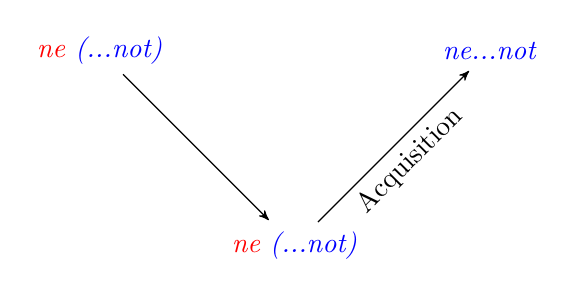
\begin{tikzpicture}[->,>=stealth',shorten >=1pt,auto,node distance=3.5cm]
      \node (C)  { \emph{\textcolor{red}{ne} \textcolor{blue}{(...not)}} };
      \node (D) [below right of=C] { \emph{\textcolor{red}{ne} \textcolor{blue}{(...not)}} };
      \node (E) [above right of=D] {\emph{\color{blue} ne...not} };
      \path[->] (C) edge node[sloped, anchor=center, below] {} (D)
      (D) edge node[sloped, anchor=center, below] {Acquisition} (E);
    \end{tikzpicture}
  \end{center}
	\caption{Syntactic acquisition as the cause of the first transition}
	\label{first-acquisition}
\end{figure}

So, the upper left \emph{\textcolor{red}{ne} \textcolor{blue}{(...not)}} indicates grammatical knowledge that includes both the pre-verbal and embracing form. But, there is no increase in the embracing form due to use. We indicate the increase in the embracing form due to acquisition as the upwards arrow in Figure \ref{first-acquisition}. The result of acquisition is that only the embracing form is acquired.  Again, while we only show a single step, this could just as well be the result of several iterations. Crucially, it is acquisition rather than use that is driving the increase in the embracing form. 

While we can present these two causes in isolation, another possibility is that both use and acquisition interact over time, giving rise to the embracing form. However, the important thing in any case is the form that an explanation must take. That is, for pragmatic use or syntactic acquisition to serve as explanations of the first transition we must demonstrate how they cause the increase in the frequency of the embracing form. We need a model of use or acquisition that makes both qualitative and quantitative predictions. That is, we need a model that predicts \emph{that} the first transition will happen, as well as \emph{how} it will happen.

The same requirements holds for the second transition.  We can represent what a pragmatic or syntactic explanation would like in Figures \ref{second-pragmatic} and \ref{second-acquisition}. For either to serve as an explanation, we would have to demonstrate how they cause the increase in \emph{\color{green} not} over time. Note that these requirements are independent of whether it makes sense to conceive of the second transition as a push-chain or whether we think that use or acquisition play any role whatsoever. In fact, it serves as an important check on any models we posit for the first transition. For example, if we have no reason to think that pragmatic use is what drives the second transition, then a model of the first transition based on use should not predict the second transition. 

\begin{figure}
  \begin{center}
    \begin{tikzpicture}[->,>=stealth',shorten >=1pt,auto,node distance=3.5cm]
      \node (C)  { \emph{\textcolor{blue}{(ne...)} \textcolor{green}{not}} };
      \node (D) [below right of=C] { \emph{\color{green} not} };
      \node (E) [above right of=D] {\emph{\color{green} not} };
      \path[->] (C) edge node[sloped, anchor=center, below] {Use} (D)
      (D) edge node[sloped, anchor=center, below] {} (E);
    \end{tikzpicture}
  \end{center}
	\caption{Pragmatic use as the cause of the second transition}
	\label{second-pragmatic}
\end{figure}


\begin{figure}
  \begin{center}
    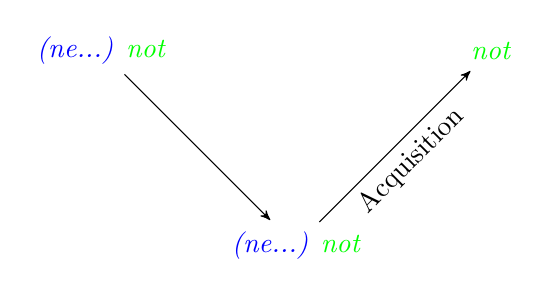
\begin{tikzpicture}[->,>=stealth',shorten >=1pt,auto,node distance=3.5cm]
      \node (C)  { \emph{\textcolor{blue}{(ne...)} \textcolor{green}{not}} };
      \node (D) [below right of=C] { \emph{\textcolor{blue}{(ne...)} \textcolor{green}{not}} };
      \node (E) [above right of=D] {\emph{\color{green} not} };
      \path[->] (C) edge node[sloped, anchor=center, below] {} (D)
      (D) edge node[sloped, anchor=center, below] {Acquisition} (E);
    \end{tikzpicture}
  \end{center}
	\caption{Syntactic acquisition as the cause of the second transition}
	\label{second-acquisition}
\end{figure}


\section*{Summary}

In this chapter we made the important terminological distinction between the formal and functional Jespersen cycles and noted the logical relationship between the two phenomena. An explanation of the formal cycle requires an explanation of the functional cycle, but not vice versa. importantly, given that the functional cycle can occur independently of the formal cycle, an explanation of the first may be fundamentally different from an explanation of the second. This guides our approach to explaining the two processes in the history of English, observed as the transitions from \emph{\textcolor{red}{ne}} to \emph{\color{blue} ne...not}  to \emph{\color{green} not}. 

In Part I we pursue an explanation of the functional cycle based on pragmatics. We present a mathematical framework for modeling how meaning is signaled in a population over time and apply it to modeling how pragmatic use leads to the transition from \emph{\textcolor{red}{ne}} to \emph{\color{blue} ne...not}, but not the transition from  \emph{\color{blue} ne...not}  to \emph{\color{green} not}. In Part II we turn to the formal cycle as a whole and evaluate whether a model of syntactic acquisition can explain either of the transitions, from \emph{\textcolor{red}{ne}} to \emph{\color{blue} ne...not} and from \emph{\color{blue} ne...not}  to \emph{\color{green} not}.

% Bibliography
\bibliographystyle{mcbride}
\bibliography{ahern}

\end{document}